\chapter{Background}


Functional programming uses immutable values and mathematical functions, also known as pure functions, to build programs. Similarly to imperative procedures, pure functions take parameters as input and produce some output. In fact, pure functions are only allowed to transform their inputs to outputs and cannot have any other observable effect. A pure function must always evaluate to same outputs, given the same inputs. Abstraction and reuse, similarly to in imperative programs, is achieved by composing a group of functions into larger functions. Composition is done by repeatedly passing the output of the previous function to the next function's input. The entire program can be seen as large function composition of all functions used in the program.

Even though imperative programming and functional programming might seem to be quite similar at first, they differ significantly. Any expression in functional programming can always be \textit{substituted} with its value without changing the meaning of the program. The same is not true in imperative programming. There is an implicit temporal coupling between imperative statements, since a statement may depend on the state set by previous statement. Because of this, reordering procedure calls or substituting any procedure call with its return value might completely change the meaning of the program.~\cite[Chapter~1]{sicp}

A program is considered to be \textit{referentially transparent} if it is possible to substitute an arbitrary expression in the program with its corresponding value without changing the meaning of the program in any way. Referentially transparent programs are easier to understand since they enable \textit{equational reasoning}, also known as \textit{local reasoning}. When working with a pure function, one does not have to understand its implementation, because the only effect the function is allowed to have is to return a result. A developer can only focus on the \textit{function's signature}, that is, what are the inputs and what is the output. Compilers can also take advantage of referential transparency by safely reordering expressions, evaluating expressions at compile time, memoizing results or by completely skipping the evaluation of expressions that are not required.

Referential transparency is one of the biggest distinguishing factors between functional and imperative programming. Abandoning referential transparency has wide-reaching implications. In practice, it makes it much more difficult to refactor and develop the program. Developers are required to be disciplined and to have wider knowledge of the whole program in order not to unintentionally cause defects. This is even more evident when programming in the presence of concurrency, which could lead to race conditions and hard to reproduce errors.~\cite[Chapter~3]{sicp}

This chapter first introduces what effects are and discusses certain common effects in more detail. Then, different ways of managing and including effects into a programming language are presented. These include unrestricted side effects and effect systems, as well as more advanced techniques such as monadic effects and algebraic effects and handlers. Finally, the history and features relevant to managing side effects of the Scala programming language are introduced.


\section{Effects} \label{effects}
Constructing practical programs and applications only by composing pure expressions without any notion of impurity is quite limiting to say the least. If the sole purpose of an expression is not to evaluate to a value or if its evaluation requires interacting with the outside world, the expression is said to have an effect. For example printing to the console, accessing the system clock or doing IO are all examples of effects. There is no unambiguous and exact definition of what an effect is, although the concept has been given, somewhat differing, characterizations by many.

\textcite{den-lang-specs} suggest that \textquote{A complete program is thought of as an agent that interacts with the outside world, e.g., a file system, and that affects global resources, e.g., the store [mutable memory]}. They continue by stating that every phrase in a program could be classified to either a value or an effect. A value is a referentially transparent expression, while an effect is an interaction with resources allocated for the program. When an effect is encountered, the control is transferred to a \textquote{central authority}. The central authority manages the use of all resources the program has access to. They continue to describe the interaction between an effect and the central authority
\begin{displayquote}
An effect is most easily understood as an interaction between a sub-expression
and a central authority that administers the global resources of a program. (..) Given an administrator, an effect can be viewed as a message to the central authority plus enough information to resume the suspended calculation.
\end{displayquote}

\textcite{imperative-fp} as well as \textcite{do-be-do-be-do} see the distinction between expressions and effects as \textit{being} vs. \textit{doing}. \rly{This observation is quite interesting since it brings up the concept of computations as values.} Certain approaches consciously differentiate computations from values, while some consciously unify them. It is later discussed how separation of effects from values applies to monadic effects and algebraic effects with handlers, together with the concept of central authority presented earlier.

\todo{Internal vs external effects ?}
% https://www.youtube.com/watch?v=G8XMRZKOhG0&t=2659s


\subsection{Mutability} % Pitäisikö olla mielummin "Mutable state"
Mutability means that the program is able to change the state of the program, usually by mutating data stored in some memory location, and state change is possible to be detected by observing the changed value. The existence of several control structures and language features require mutability. The destructive assignment operation found in almost every mainstream language is by definition mutation.~\cite[Chapter~3]{sicp} Looping constructs like for- and while loops or iterators found in many standard libraries rely heavily in the notion of mutation. Also parts of some well known algorithms, like swap operation in quicksort, could be expressed trivially as mutation.

In practice, almost all applications have some state that determines how the application reacts to new input. The concept of state is naturally and in the most straightforward way represented by starting with an initial state and then mutating it as the execution of the program continues. Real-world examples of state are the location of characters in a game, registered users in an application or cursor position in buffer when reading bytes from a socket. In the presence of concurrency, when parallel computations are expected to interact with each other, mutability in one form or another is needed to indicate if the computation is still on-going, completed or have encountered an error.

% Kerro muuttuvan jotain tilan semantiikasta ?
% - Teoreettinen pohja ? (side-effects T A = (A × S))


\subsection{Exceptions} \label{effects:exceptions}
Another very common effect is the ability to signal about exceptional conditions where the program is unable to compute a result or execute a command. This signaling is achieved by raising an error or exception. An exception could contain information about the condition that caused it, for example malformatted input, and that could possibly be later used when \textit{handling} or recovering from the exception. There are several common reasons for exceptions to arise, they usually fall into two categories: technical or logical. Logical exceptions can be seen as a way for a function to have an alternative return value.~\cite{imprecise-exceptions}

Logical exceptions are usually caused by failing to meet some preconditions regarding the program's state or function's parameters. A function may have assumptions about its inputs, maybe a string must be in a format corresponding to a schema in order to parse it successfully, or an integer must be positive and less than certain threshold to represent a year. Sometimes inputs must be compatible with other inputs, an example of such case is accessing an array by its index where the accessed index must be less than or equal the size of the array, or a user may attempt to access authorized content before proper authentication and authorization process.

Technical exceptions can further be separated into synchronous and asynchronous exceptions. Peyton Jones describes that synchronous exceptions "arise as a direct result of some piece of code".~\cite{akward-squad} These exceptions are usually caused by problems related to IO, runtime environment, or the programming language itself. In the other hand, asynchronous exceptions are caused by external events and they cannot always be tied to the execution of a particular line of code. In some way, logical and synchronous exceptions are expected exceptions, and asynchronous exceptions are unexpected.

A large part of synchronous exceptions are related to IO. If attempting to interact with a file that does not exist or the current permissions are not sufficient, the result will likely be an exception of some sort. One significant source of exceptions is communicating over the network with a remote party. Everything from name resolution, routing, transport protocol or communication schema could go wrong. A remote component in a distributed system could be completely unavailable due to network error or internal error in that specific component. Other types of IO problems are trying to perform an action before initialization of for example via a database connection, file descriptor or IO port.

Other synchronous exceptions may be caused by division by zero or a non-exhaustive pattern match. Probably the most well known synchronous exception is the infamous null reference error, where the program is trying to dereference a pointer that does not point to valid memory location. In languages that support direct memory access, an attempt to access memory outside of the allowed memory range leads in a program or operating system level exception.~\cite{akward-squad}

Asynchronous exceptions usually originate from the runtime environment of the program, operating system, concurrency, or user interruption. Asynchronously raised exceptions are characterized by the fact that they could occur at an arbitrary point in time.~\cite{async-exc} An example of this is a situation where a thread interrupts the execution of another thread. The whole program could also be interrupted by a user (for example by pressing Ctrl+C) or the runtime, possibly due to a critical error in the program or operating system. Resource exhaustion is another common cause of asynchronous exceptions. Errors like stack overflow or out of memory can happen every time new memory is required from the stack or heap, thus those are categorized as asynchronous. Many environments also support dependencies to libraries that are loaded/linked  dynamically at run time. It is not always possible for the programmer to determine the exact time of when dynamic loading should happen, and for this reason failing to load required dependencies could be considered an asynchronous exception.~\cite{akward-squad}

Exceptions can also encode another related and important concept, \textit{optionality}. Encoding it via exceptions is achieved by raising an exception that contains only a value of unit type\footnote{A type whose cardinality is 1 (i.e., that has only one value) and thus does not contain any information.}, signaling that a result could not be computed and there is no additional information about the exception. Optionality is an approriate choice instead of exceptions when the cause of the exception is trivial. Such cases include unsuccessfully querying a row from a database with specific id, searching an element from array or trying to find a substring from a string.

Usually, the semantics of raising and handling an error are considered to interrupt the normal control flow of the program and transferring the execution to the closest appropriate \textit{exception handler}. An exception handler decides if and how to continue the execution, or whether to let the exception bubble up the layers of exception handlers. This "short-circuiting" semantics is a natural way to think and program in the presence of errors. However, the ability to raise errors from an arbitrary location can make it difficult to understand the meaning of the program and prove its correctness. It also poses challenges to ensure that any exceptions that may be raised are handled appropriately. Lazy evaluation complicates things even further. A lazily evaluated language does not have an unambiguous control flow since values are computed only when required. This makes it harder to define clear semantics for exceptions.~\cite{imprecise-exceptions}

Effective and thorough exception handling is one of the most important practices in successful software engineering. Conversely the inability to do so is one of the most significant factors that causes bugs and failures in software systems. A 2014 study by the University of Toronto studied multiple popular open source distributed software systems, such as Redis, Hadoop and Cassandra and found that a large portion (35\%) of catastrophical failures are caused by trivial mistakes in error handling code. Such mistakes include practices like omitting error handling code completely and writing a TODO-comment instead. In addition to failures, inadequate error handling may expose security vulnerabilities in the system.~\cite{simple-testing-failures}
% - Teoreettinen pohja ? (exceptions T A = (A + E) + kyky keskeyttää control flow)


\subsection{Continuations, Concurrency \& Asynchrony}
\todo{Onko "oikea" effect ja tarviiko omaa lukuaan?}
\todo{Voisi olla hyödyllistä mainita blocking/continuation ja CPS ?}
% Tässä voisi viitata "What color is your function" ?
%   - https://journal.stuffwithstuff.com/2015/02/01/what-color-is-your-function/


\subsection{IO}
Programs need the ability to interact with the external world.
A program could interact with a user, other programs, or devices and sensors. IO is the medium to carry out these interactions. Like interaction in general, IO is most often bidirectional - the term IO is shorthand for input and output. Input is the ability observe changes and to receive information from other parties, output enables the program to cause changes in the environment and to dispatch information to others.

Many IO effects are about interacting with the user. Probably the most well-known and fundamental form of user interaction is to display text and graphics by changing pixels on the screen. Another common type of user interaction is via the console, which consists of printing characters to standard output and reading user input from standard input. The use of external devices such as playing sounds from speakers, recording sound from a microphone, or receiving user input from the keyboard, mouse, and touchscreen, is essential in user interaction.

In addition to user interaction, the program can also use devices for other purposes. For example, reading the time from the system clock, requesting the current temperature from a sensor, or setting a digital output to 1 or 0. Communicating with other programs is also established by utilizing a capable device. These devices usually connect to a network or bus that transmits bits between different parties. In addition, these devices often encapsulate the low-level details of a specific communication protocol.

Often programs need the ability to store data that persists even when the program is restarted. This is achieved by using a device that allows reading from and writing to a non-volatile memory, such as a hard drive or memory card. Many times the operating system abstracts this persistent data store by providing a file system. However, many embedded devices still communicate directly with the persistent memory device.

The reason for a program to exist is to eventually have an effect on the surrounding world. As IO is the only way to achieve this, it fundamentally distinguishes IO from other effects. Where other effects might be useful when implementing programs, IO is \textit{the reason} for programs to exist in the first place.~\cite{akward-squad} To put it other way around, it would be impossible to detect if program is running or not if it would not be interacting with its environment.


\section{Unrestricted side effects}
The most straightforward way to incorporate effects into a programming language is by not giving them any special treatment. This way pure expressions and effectful statements are treated equally and could be combined with each other in any way. Evaluation of any method, function or procedure could cause side effects to occur. This gives the programmer a lot of freedom when implementing an application, as the language does not place constraints on how parts of the code could be composed. Another consequence of this approach is that the programmer is solely responsible for managing effects and making sure that they are compatible with each other. Even a small change in a program could cause unintentional side effects to occur.

In the industry today, unrestricted side effects are the default way to incorporate effects into a programming language. Virtually all mainstream programming languages allow unrestricted side effects in one way or another. This is probably because the majority of the mainstream languages originate from the C family of programming languages that are essentially imperative. Although the benefits of static typing are widely recognized, typing of effects has not yet been added to any mainstream language.


\section{Effect systems}\label{effects:effect-systems}
\todo{Korosta että kun ohjelmoidaan effectien kanssa, halutaan tietää mitä effectejä (exceptions, (mutable)state, continuations) kullakin expressionilla on. Effect system hoitaa tämän}
The purpose of an effect system is to allow mixing effectful and pure code safely. The idea of an effect system is very similar to that of a type system. In some programming languages, a type system can even be used to implement an effect system, or in others they are two separate systems. A type system sets the rules according to which functions, parameters, expressions, and, in some cases, objects can be composed. Static type system also checks that these rules are obeyed before the program is run.

Effect system enforces rules what effects expressions and statements have, and how these effects can interact with each other. Similarly to type systems, these interactions are checked statically at compile-time. Like a type system, an effect system can require the programmer to specify intended effects for every function/expression, or in some cases infer them from the context. Contrary to type systems where an expression usually evaluates to a single type, effects of an expression could be seen as a set of effects used by the expression. Empty set of effects denotes an expression that is free of effects.

Research related to statically checking effects began to be active in the mid 80s and 90s. Even earlier first efforts in this direction were the Pascal extensions Euclid (in the 70s) and Ada (in the 80s) that separated side effecting procedures from pure functions~\cite{real-prog-in-fp}. The term effect system was introduced by \textcite{intgr-fp-ip} in \citeyear{intgr-fp-ip}. Their idea was to assign different \textit{effect classes} to different parts of a program. The paper proposed rules how these different classes are allowed to interact with each other. For example, a pure function is not allowed to call a function that is labeled with a more permissive effect class. This would allow to safely mix functional and imperative code while preserving equational reasoning of the functional parts and tracking possible effects of the imperative parts. In the paper, the only effectful operations were related to allocating, mutating and reading memory locations. The initial goal was to determine what parts of the program could be run in parallel without changing the semantics of the program.

Probably the most widely known application of effect systems is checked exceptions in Java (\refsource{java-checked-exc}). This part of Java's type, or effect, system is only concerned of tracking exceptions, more specifically where they are thrown and catched. If a method might throw an exception, it must be declared in a \inlinecode{throws} clause in the method's type signature. The compiler forces any code that calls the method to either handle the exception or to add a \inlinecode{throws} clause to indicate that the exception will bubble up. Checked exceptions has been widely criticized for making programming clumsy, and nowadays it is common for the whole feature to be circumvented when possible.

\begin{algorithm}

\begin{minted}{java}
public byte[] readFile(String fileName) throws IOException {
    var file = new File(fileName);
    var is = new FileInputStream(file); // can throw IOException
    return is.readAllBytes();           // can throw IOException
}

public void catchIt() {
    try { var bytes = readFile("file.txt"); }
    catch (IOException exc) { /* Handle error  */ }
}

// Caller must handle IOException
public void declareIt() throws IOException {
    var bytes = readFile("file.txt");
}
\end{minted}

\caption{Checked exceptions in Java. \label{java-checked-exc}}
\end{algorithm}

Since their introduction, effect systems have evolved significantly and gained more sophisticated features such as the ability to track non-memory related effects like IO and exceptions. Several effect systems~\cite{koka-lang, frank-lang} allow the user to define custom effect types. Effect polymorphism~\cite{polymorphic-alg-effs}, which allows to express effectful higher-order functions safely and conveniently, has also been actively researched and developed. Modern languages with built-in effect systems~\cite{unison-lang, ocaml-lang} usually include algebraic effects and handlers, which are discussed in more detail in section \ref{background:alg-eff}. Library-level support for effect systems is commonly based on monadic effects, which are discussed in section \ref{background:monads}.

% Gifford and Lucasse introduced 'effect systems' which use types to record the side-effects performed by a program, and to determine which components of a program can run in parallel without interference.
%   - Imperative functional programming p. 12, ch. 7.1

% But effect systems are designed for impure,. strict functional languages, where the order of sequencing is implicit. Our work is designed for pure, lazy functional languages, and the purpose of the 'bind' operation is to make sequencing explicit where it is required.
%   - Imperative functional programming p. 13, ch. 7.1



\section{Scala} \label{background:scala}
Scala is a high level, statically typed, multi-paradigm, compiled, and garbage collected programming language. Eager evaluation is the default, but lazy evaluation is also supported. It is most commonly run on \acronym{JVM}{Java Virtual Machine}, but also JavaScript and native code are supported compilation targets. The first release was in 2004 and the latest version is 3 which was released in 2021. Scala 3 is exclusively used in this thesis. The initial and current lead designer of the language is Martin Odersky, a professor at the École polytechnique fédérale de Lausanne, meaning that Scala has its roots in an academia, although its approach is pragmatic.

Scala aims to blend functional and \acronym{OOP}{Object-oriented programming} paradigms and as a result has features from both paradigms. Many OOP concepts like classes, objects, interfaces and polymorphism are supported. In fact, every value in Scala is an object. Scala uses class-based objects with attributes and methods as well as enables multiple inheritance. Scala supports generics with lower and upper type constraints as well as declaration-site variance. The language also includes many imperative constructs like loops and mutable variables that are commonly used in other OO-languages. In Scala everything is an expression, including control structures like \inlinecode{if/else}, \inlinecode{try/catch}, and loops. \refsource{scala:basics} demonstrates the basic syntax of Scala.

\begin{algorithm}

\begin{minted}{scala}
trait Foo // Define an interface
class Bar extends Foo // Define a class inheriting from Foo

// Define variables/constants
var mutableFoo: Foo = Bar() // Explicit type is Foo
val immutableBar    = Bar() // Inferred type is Bar
lazy val lazyPlus   = 1 + 1 // Computed lazily and cached

// Type argument here is Int
val genericType: List[Int] = List(1, 2, 3)

// Type parameters are declared between '[' and ']'
def genericMethod[A](a: A): A = a

// Type parameter constraints:
// 'A' must be supertype of 'Bar' and  'B' must be subtype of 'Foo'
def typeBounds[A >: Bar, B <: Foo](a: A): B = ???

// ??? is defined in the standard library. It can replace any
// expression; it's type is Nothing, the bottom type
def `???` : Nothing = throw new NotImplementedError

// => specifies 'by-name' calling convention:
// The parameter n is evaluated every time it is used (2 times here)
def byNameParameter(n: => Int) = n + n
\end{minted}

\caption{Basic syntax of Scala. \label{scala:basics}}
\end{algorithm}

Due to Scala's object-oriented nature, every object is part of a type hierarchy. On top of the hierarchy is \inlinecode{Any}, which is the supertype of all other types. Below \inlinecode{Any} is \inlinecode{Matchable}, which marks type suitable for pattern matching. \inlinecode{Matchable} has two subtypes: \inlinecode{AnyVal}, which is a supertype for all value types, and \inlinecode{AnyRef}, which is a supertype for all reference types. \inlinecode{Null} is subtype of all reference types, except when \textit{explicit nulls} -feature is enabled and \inlinecode{Null} becomes subtype of \inlinecode{Any}. Scala also has a bottom type \inlinecode{Nothing}, that is subtype of every type. No values of type \inlinecode{Nothing} could ever exist at runtime so the type reflects the absence of value, for example in the case of infinite recursion, loop, or when the expression throws an exception. Diagram in Figure \ref{fig:scala-type-hierarchy}, demonstrates the type hierarchy.

\begin{figure}
    \centering
    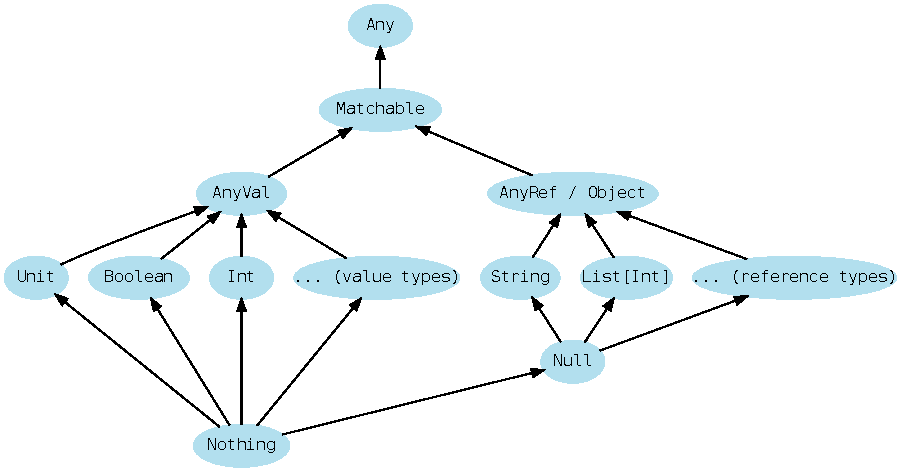
\includegraphics{images/type-hierarchy}
    \caption{Scala 3 type hierarchy}
    \label{fig:scala-type-hierarchy}
\end{figure}

\todo{Pitäisikö varianssin olla irrallinen Scala-kappaleesta?}
Variance defines the rules how subtype relationship between parameterized types are dependent on the subtype relationship on the type on which it is parameterized. Variance has three variants: \textit{invariance}, \textit{covariance}, and \textit{contravariance}. Invariance means that subtyping relationships present in the type parameters are not applied to the parameterized type at all. Covariance states that subtype relationship of the parameterized type are in the same direction as the type parameter's subtype relationship. In the other hand, contravariance means that the subtype relationships between parameterized types are the opposite way compared to the subtype relationships of the type parameter. A parametric type with multiple type parameters could declare each type parameter with different variance, for example functions in Scala are contravariant in their input type(s), and covariant in their result type. When \inlinecode{Sub} is subtype of \inlinecode{Super} and \inlinescala{F[_]} is any parameterized type, then:
\begin{itemize}
    \item Covariance: \inlinescala{F[Sub]} is subtype of \inlinescala{F[Super]}
    \item Contravariance: \inlinescala{F[Super]} is subtype of \inlinescala{F[Sub]}
    \item Invariance: \inlinescala{F[Sub]} and \inlinescala{F[Super]} have no subtyping relationship
\end{itemize}

Covariance is applicable in parameterized types that contain, store, or produce values, in other words the type parameter is in covariant position. Contravariance is applicable in the opposite situation, where values of the type parameter are consumed, i.e. the type parameter appears in a function parameter list, and is said to be in contravariant position. Invariance is useful in situations where it does not make sense for the parameterized type to have inheritance based on type parameter, or when the parameterized type is a mutable, or the type parameter appears both in covariant and contravariant positions.

An infamous example of mutable covariant type is primitive array in Java and C\# that perform a runtime type check when adding elements to the array, and throw exception if the type of the element is not compatible with the array, as demonstrated in \refsource{mutable-covariance}.
To avoid similar situation, mutable collections in Scala are invariant. Immutable collections and containers, such as \inlinecode{Option} or \inlinecode{Either} are covariant in Scala.

\begin{algorithm}

\begin{minted}{java}
String[] a = new String[1];	
Object[] b = a; // String is a subtype of Object, so this is legal
b[0] = 1; // Runtime exception since cannot add Integer to String[]
\end{minted}

\caption{Covariance in mutable types, like Java primitive array, is problematic \label{mutable-covariance}}
\end{algorithm}

Programming languages differ in the way the variance is defined. Languages like C\# and Scala define the variance with the parameterized type. In the other hand, language like Java define the variance only when using the parameterized type. The former is called \textit{declaration-site} variance, demonstrated in \refsource{declaration-site-variance} and the latter is called \textit{use-site} variance, demonstrated in \refsource{use-site-variance}. Approaches deviating from these exist, for example TypeScript does not have explicit variance notation at all, and relies on inferring the variance. Invariance is the default in Scala and does not require explicit denotation. Covariance is declared with a \inlinecode{+} sign before each type parameter. Since contravariance could be seen as the opposite of covariance, it is denoted with a \inlinecode{-} sign.

\begin{algorithm}

\begin{minted}{scala}
class Invariant[A]      // Invariance is the default
class Covariant[+A]     // Covariance denoted with +
class Contravariant[-A] // Contravariance denoted with -
\end{minted}

\caption{Scala uses declaration-site variance, where the variance of a parameterized type is denoted in its type definition  \label{declaration-site-variance}}
\end{algorithm}

\begin{algorithm}

\begin{minted}{java}
interface Supertype {}
interface Subtype extends Supertype {}

void invariant(List<Supertype> list) {
    /* Get and set list values */
}
void covariant(List<? extends Supertype> list) {
    /* Only get list values */
}
void contravariant(List<? super Subtype> list) {
    /* Only set list values */
}
\end{minted}

\caption{Java has use-site variance, where the desired variance is declared when using the parameterized type \label{use-site-variance}}
\end{algorithm}

Many features and principles from functional programming are not only available, but also encouraged in Scala. Pattern matching, first-class functions (\refsource{scala:lambdas}), and tail recursion are all supported and heavily utilized in idiomatic Scala programs. Immutable variables, collections and data-structures are default the default way of writing Scala, even though mutable counterparts are also available. Functional data modeling is achieved with the use algebraic data types built into the language. Even though Scala embraces functional programming and imperative code is generally discouraged, introducing arbitrary side effects is possible.

\begin{algorithm}
\begin{minted}{scala}
val ns = List(1, 2, 3)

val mapped1 = ns.map(n => n + 1)
val mapped2 = ns.map(_ + 1) // Same as above in shorter form

val sum1 = ns.foldLeft(0)((x, y) => x + y)
val sum2 = ns.foldLeft(0)(_ + _) // Same as above in shorter form
\end{minted}

\caption{Long and short form of anonymous functions in Scala. \label{scala:lambdas}}
\end{algorithm}

In addition to ordinary functions, Scala has specific function called \inlinecode{PartialFunction} that is not defined for all values of its input type. It is a subtype of normal function and adds method \inlinecode{isDefinedAt}, which must be used to check before every function call whether the function is defined for the given value. Usually partial functions are not called directly by the programmer, but rather they are utilized in libraries to create better APIs. Partial functions are useful in pattern matching and many collection operators, such as \inlinecode{collect}, present in all standard library collections, which could be used instead of sequential \inlinecode{map} and \inlinecode{filter} operations. \refsource{scala:partial-function} shows how to define and use partial functions.

\begin{algorithm}
\begin{minted}{scala}
val someEvensMultipliedByTen: PartialFunction[Option[Int], Int] = {
  case Some(n) if n % 2 == 0 => n * 10
}

val opts  = List(None, Some(2), None, Some(3), Some(4))
val somes = opts.collect(someEvensMultiplied) // List(20, 40)
\end{minted}

\caption{Partial functions in Scala. \label{scala:partial-function}}
\end{algorithm}

Some functional languages, such as Haskell, have a special syntax for monadic computations. Scala also provides this syntactic sugar in a form of \inlinecode{for} comprehensions, demonstrated in \refsource{monad:for-syntax}. For comprehension is compatible with any data type that has \inlinecode{map} and \inlinecode{flatMap} methods defnied, such as \inlinecode{Option}, \inlinecode{Either}, and \inlinecode{ZIO} (chapter \ref{zio}). One could also add required methods to any type by using extension methods.

Being a academic language, Scala also has quite a lot more advanced features. Starting from extension methods, which enable to add methods to a class separately from its definition, operator overloading and infix operator- and method syntax, all the way to higher kinded and dependent types, type lambdas, as well as powerful meta programming capabilities. Scala 3 introduced more advanced features such as automatic type class derivation and union and intersections types.

Probably the most distinguishing feature in Scala is its implicit system and other contextual abstractions arising from that. Function could mark some of its parameters as implicit and the compiler would try to find that paramater from the enclosing scope by its type without programmer explicitly passing it as a parameter. Originally implicit parameters were introduced to achieve similar behavior as Haskell's type classes. Implicits could also be used for other purposes such as implicit conversions, context propagation, extension methods, and proving subtyping relationships between generic type parameters at compile-time.~\cite{tc-as-objects}

Function can mark some of its parameters as implicit with the keyword \inlinecode{using}. When the function is called, the compiler tries to find a value marked as implicit, with the keyword \inlinecode{given}, from the enclosing scope. If all requested values are found, they automatically inserted as parameters. If any of the implicit parameters is not found, an compilation error is reported. \refsource{scala:implicits} demonstrates function \inlinecode{summon}, which simply searches for implicit value by type, and the definition and usage of implicit parameters.

\begin{algorithm}
\begin{minted}{scala}
case class Person(age: Int, name: String)

// Define type class
trait Show[A]:
  extension (a: A) def show: String

// Define type class instance
given Show[Person] with
  extension (a: Person)
    def show: String = s"${a.name} is ${a.age} years old"

// Use the type class
def showAll[A: Show](as: List[A]): List[String] =
  as.map(a => a.show)
\end{minted}

\caption{Implicits could be used to encode type classes \label{scala:typeclasses}}
\end{algorithm}

Another advanced feature utilizing implicit resolution, is the ability of the Scala compiler to prove type equality or sub type relationships. There are two classes \inlinescala{=:=[From, To]} for type equality and \inlinescala{<:<[From, To]} for sub type relationship. Both classes extend a function \inlinescala{From => To}, and can be used to transform types. Types with two type parameters could be used as infix in Scala, for example type equality could be written \inlinescala{A =:= B}. When requesting implicit parameter of either of the types above, Scala compiler synthesizes an instance if the type relationship holds, otherwise reports a compilation error. The act of proving type relationships is said to be \textit{witnessing}, and a common practice is to name the implicit parameter as \textit{evidence}. The feature is useful, for example, when defining functions that make sense only for specific types, as demonstrated in \refsource{scala:witness}, where only nested \inlinecode{Maybe} types could only be flattened.

\begin{algorithm}
\begin{minted}{scala}
enum Maybe[+A]:
  case Just(a: A)
  case Nothing

  def flatten[B](using evidence: A <:< Maybe[B]): Maybe[B] =
    this match
      case Just(a) => evidence(a)
      case Nothing => Nothing

Maybe.Just(Maybe.Just(1)).flatten // Compiles
Maybe.Just(1).flatten // Error: Cannot prove that Int <:< Maybe[B]
\end{minted}

\caption{Scala compiler can prove (witness) a subtype relationship by providing implicit evidence. \label{scala:witness}}
\end{algorithm}

Another thing that sets Scala 2 and 3 apart is the introduction of intersection and union types in Scala 3. Intersection types are denoted with \inlinecode{&} symbol and union types with \inlinecode{|}. Intersection \inlinescala{A & B} means that the resulting type has properties of both \inlinecode{A} \textbf{and} \inlinecode{B}. Union is the dual of intersection, and the resulting type of \inlinescala{A | B} is either \inlinecode{A} \textbf{or} \inlinecode{B}.

Intersection types are commutative, idempotent, and have \inlinecode{Any} as the identity element. Commutativity means that the order of types included in the intersection does not matter, and Scala considers permutations equal. Idempotency states that type in intersection with itself is equal to the type itself. \inlinecode{Any} as the identity element means that the intersection of any type \inlinecode{A} with \inlinecode{Any} is equal to \inlinecode{A}, since all types themselves are subtypes of \inlinecode{Any}. Laws of intersection types witnessed by the Scala compiler:
\begin{itemize}
    \item Commutativity: \inlinescala{summon[(A & B) =:= (B & A)]}
    \item Idempotency: \inlinescala{summon[A =:= (A & A)]}
    \item Identity: \inlinescala{summon[A =:= (A & Any)]}
\end{itemize}

Like intersection types, also union types are commutative, idempotent, and have \inlinecode{Nothing} as the identity element. \inlinecode{Nothing} as the identity element means that the union of any type \inlinecode{A} with \inlinecode{Nothing} is equal to \inlinecode{A}, since there is no values of type \inlinecode{Nothing}. Laws of union types witnessed by the Scala compiler:
\begin{itemize}
    \item Commutativity: \inlinescala{summon[(A | B) =:= (B | A)]}
    \item Idempotency: \inlinescala{summon[A =:= (A | A)]}
    \item Identity: \inlinescala{summon[A =:= (A | Nothing)]}
\end{itemize}


\subsection{Capture checking}
Scala 3 is based on a research language called Dotty. The name Dotty comes from \acronym{DOT}{Dependent object types}, which is the theoretical foundation behind Scala 3~\cite{essence-of-dot}. While writing the thesis, feature called Capture checking~\cite{capture-checking} was added to Dotty and later to Scala 3 as an experimental feature. The idea of capture checking is to enable effectful programming in direct style (discussed in section \ref{background:monad:syntax}), while tracking effects in the type system and providing strong static guarantees of the correctness of the program.

\textcite{scoped-capabilities} published a paper that describes their findings regarding modeling polymorphic effects with capabilities. The initial version of capture checking is based on their work. \todo{Onko viittaus järkevä?} In the paper, they criticize the currently widely used ways of managing effects, such as Java checked exceptions and monads, as lacking in both usability and flexibility, that result in complex and duplicated code. They conclude that this is due to the transitive nature of effects in function call chains, combined with the classical type-systematic approach that \textquote{characterize the shape of values but not their free variables}, and suggest that modeling effects with capabilities may circumvent the problems they described.

The goal of capture checking is to address many of the limitations in effectful programming. These include how to solve the "What color is your function" problem~\cite{what-color-is-your-function}, how to express effect polymorphism, how to combine manual and automatic memory management, how to express high-level concurrency and parallelism safely, and how to migrate already existing programs to this new style~\cite{odersky-twitter-caprese}. ~\todo{Voiko lähdeviittaus olla Twitteriin, koska vaikuttaa että tavoitteet listataan julkisesti ainoastaan siellä} The research focuses on the usability aspect of static effect tracking, which likely will evolve around effect polymorphism, inferring the the captured capabilities, direct style of programming, and in general minimizing the overall syntactic overhead.

Capture checking aims to address effects such as throwing exceptions, IO, mutability, and suspending computations and continuations. Resources are similar to effects but have some distinct properties. Resources, such as file handles, network connections, or memory) must be acquired before use, and disposed afterward to possibly clean up to free up OS level resources. This leads to the observation that a resource has \textit{lifetime} in which it could be used, and the usage of already disposed resource should be prevented. For the same reason, the sharing of resource between multiple parties requires rules. The lifetime and rules should preferably be enforced statically by the type system. This is closely related to lifetimes in Rust~\cite{rust-lifetimes} and linear type systems in general.

The fundamental idea of capture checking differs from the traditional effect system approach. Common approach with effect systems is that it annotates the effects what the execution of an expression might have. Capture checking, in the other hand, keeps track of the captured free variables in expressions. This means that capability is a normal value, like any other variable in a program, and both resources and effects could similarly be modeled in this way. In the context of capture checking, an expression is pure if it does not capture, i.e. close over, any capability. To make programming with capabilities easier, the capabilities could be implicitly passed to expressions, instead of requiring to explicitly thread capabilities through a program. The implicit system in Scala should be well suited for this task.

Capture checking can be enabled in Scala version 3.2.1 onwards with the compiler option \inlinecode{-Ycc}. Annotation \inlinescala{@capability} is used to mark a class/trait as capability that could be tracked. Captured capabilities are annotated before type annotation inside braces, e.g.: \inlinescala{val a: {capability} Int = 1}. \refsource{scala:cc-eff-polymorphism} provides a larger example by defining a effect polymorphic \inlinecode{List.map} function and demonstrating its usage. The syntax of capture checking is highly experimental and may be subject to change in the future.

\begin{algorithm}
\begin{minted}{scala}
// Compiles with dotty 3.2.0-RC1-bin-SNAPSHOT

// '{f}' Means that mapCC captures all capabilities of function 'f'
// This makes mapCC effect polymorphic since the resulting
// capabilities are solely determined by capabilities of 'f'
extension [A](xs: List[A])
  def mapCC[B](f: A => B): {f} List[B] =
    xs match
      case hd :: tl => f(hd) :: tl.mapCC(f)
      case Nil     => Nil

// Class is marked as capability by annotating it
@annotation.capability class Console:
  def printLine(x: Any): Unit = println(x)

// Required capabilites are declaired as constructor parameters
class Example(using val cn: Console):
  val numbers: List[Int] = List(1, 2, 3)
  
  // When function passed to mapCC does not capture capabilities
  // the resulting value does not capture anything
  val doubled: List[Int] = numbers.mapCC(n => n * 2)

  // Here the function passed to mapCC captures console capability
  // thus the resulting value captures the same capability
  // indicated in the type as '{console}'
  val printed: {console} List[Int] = numbers.mapCC { n =>
    console.printLine(n)
    n * 2
  }
\end{minted}

\caption{Effect polymorphism with capture checking %
\label{scala:cc-eff-polymorphism}}
\end{algorithm}


Odersky and the research group received a grant for seven researchers over five years, starting in September 2022~\cite{capture-checking-grant}. The research project is called Caprese (Capabilities for resources and effects), that will focus on universal theory of resources and effects based on capabilities. It will be interesting to see the results of the research group in the coming years.  The direction in which the research will develop remains to be seen.



\section{Type classes}
Type classes are a way to achieve ad-hoc polymorphism. They were first introduced by \textcite{ad-hoc-less-ad-hoc} in 1989 as a way to enable operator overloading in a programming language with Hindley-Milner type system. Eventually type classes were implemented in Haskell, largely based on Wadler's and Blott's proposal. A couple of years later, when applications of monads and related algebraic structures in programming were discovered~\cite{comp-lambda-monads}, type classes were a natural way to implement such algebraic structures.

Type class is an abstraction that defines behavior to some generic type. This enables one to implement highly generic functions that works with any type that is constrained to belong to type class. A type is said to be part of a type class if it has \textit{instance} of that type class. Instance of a type class contains functions and/or values that implement the behavior of the type class. Instances are defined separately from the type which for the instance is for, thus allowing to provide type class instances for third party data types if so desired. Example in \refsource{typeclass} demonstrates how type classes enable to implement polymorphic functions that work with any data type that belongs to specific type class.

\begin{algorithm}
\begin{minted}{scala}
case class Money(amount: Int)

trait Ordering[A]:
  extension (lhs: A) def <(rhs: A): Boolean

given Ordering[Money] with
  extension (self: Money) def <(that: Money): Boolean =
    self.amount < that.amount

// Compatible with any data type that has instance for Ordering
def sort[A: Ordering](as: List[A]): List[A] = as.sortWith(_ < _)

val sorted = sort(List(Money(3), Money(1), Money(2)))
\end{minted}

\caption{Definition, implementation and usage of the Ordering type class in Scala.%
\label{typeclass}}
\end{algorithm}


\section{Monads} \label{background:monads}
Of particular interest in this thesis is the algebraic structure monad. Algebraic structures are a concept that define functions that operate on some parametric type, or types, and are governed by algebraic laws. Algebraic structures are often studied through the lense of category theory, a branch of theoretical mathematics that studies objects, transformations between objects and relationships between different categories. In this thesis algebraic structures and monads in particular are approached from the perspective of computer science, and focusing on how monads are capable of encoding effects.

Functor is a transformation between two categories. In functional programming most, if not all, functors are endofunctors which are transformations from one category back to the same category. In practice endofunctors wrap some other category and allow to transform the inner category while preserving the outer category. List datatype is example of an endofunctor, because it allows to apply transformations to elements in the list, resulting in a new list. Monad is a special kind of endofunctor that is capable of collapsing a nested endofunctor structure. In the case of list, this means that every element in the list is transformed to a list, but the resulting list is not list of lists, but the inner lists are flattened. Listings \ref{functor:haskell} and \ref{functor:scala} show the definition of Functor type class in Haskell and Scala.

\begin{algorithm}

\begin{minted}{haskell}
class Functor f where
  fmap :: (a -> b) -> f a -> f b
\end{minted}

\caption{Functor type class in Haskell. %
\label{functor:haskell}}
\end{algorithm}


\begin{algorithm}

\begin{minted}{scala}
trait Functor[F[_]]:
  extension [A](fa: F[A]) def map[B](f: A => B): F[B]
\end{minted}

\caption{Functor type class in Scala 3 %
\label{functor:scala}}
\end{algorithm}

The applicability of monads for computer science was not discovered until the late 80s by \textcite{comp-lambda-monads} who described how the monad could be useful for defining semantics of effectful program. Moggi's proposed semantics extends lambda calculus in a pure way to support calculations previously considered to be impure. Later the idea of using monads to describe effectual computations was refined by \textcite{comprehending-monads}, \textcite{notions-computations} and \textcite{monads-for-fp}.

Any data type can form a monad if it has at least two capabilities: lifting any value to the context of the monad (i.e., the data type), and sequentially composing computations that act on these values. Every computation in these sequences has access to the values that previous computations may have produced. These computations produce values that are inside a data type and succeeding computations have access to. Lifting and sequencing must adhere to monad laws in order for the data type to be considered a monad. Monad laws are discussed in more detail in section \ref{monad:laws}.

In practice several data types naturally form a monad, such as \inlinecode{Array} in JavaScript with \inlinecode{of} function providing lifting and \inlinecode{flatMap} function providing sequencing~\cite{js-array}. Monads and other algebraic structures are often implemented as typeclasses, and writing programs consists of operations provided by the typeclass. This allow for writing highly abstract programs where generic types are constrained by requiring them to be part of certain type class. Definition of monad type class in Haskell and Scala are provided in Listings \ref{monad:haskell} and \ref{monad:scala}.

\begin{algorithm}

\begin{minted}{haskell}
class Functor m => Monad m where
  return :: a -> m a
  ( >>= ) :: m a -> (a -> m b) -> m b
\end{minted}

\caption{Monad type class in Haskell. %
\label{monad:haskell}}
\end{algorithm}


\begin{algorithm}

\begin{minted}{scala}
trait Monad[F[_]]:
  def pure[A](a: A): F[A]
  extension [A](fa: F[A]) def flatMap[B](f: A => F[B]): F[B]
\end{minted}

\caption{Monad type class in Scala 3 %
\label{monad:scala}}
\end{algorithm}

Composing programs of sequential instructions is nothing new compared to imperative programming. Monads, however, can control what effects are possible within such computations. The data type (i.e. monad) provides the context in which the computations are performed, and thus defines the semantics of lifting and sequencing. Different monads have different semantics and that allows encoding different effects with monads. The usefulness of monads comes from the fact that sequencing computations one after the other is such a primitive operation in any effectful program. Monads abstract this fundamental operation, and allow to define the meaning of sequentiality in the context of a specific monad. For example in a list monad, the semantics of sequencing is to perform the computation for every element in the list, and composing multiple lists will result in a cartesian product, demonstrated in \refsource{monad:bind}. Examples of other monads and their semantics are introduced in more detail later in this chapter.

\begin{algorithm}

\begin{comment}
\begin{minted}{haskell}
name :: IO ()
name =
  putStrLn "What's your name?" >>= \_ ->
  getLine >>= \name -> 
  putStrLn ("Nice to meet you " ++ name)
\end{minted}
\end{comment}


\begin{minted}{haskell}
suits = ["Club", "Heart", "Diamond", "Spade"]
ranks = [2..14]

-- [("Club", 2), ("Club", 3), ... ,("Spade", 13), ("Spade", 14)]
deck =
  suits >>= \suit ->
  ranks >>= \rank ->
  return (suit, rank)
\end{minted}

\caption{Monadic bind in list monad results in a cartesian product %
\label{monad:bind}}
\end{algorithm}

Even though the naming of the lifting and sequencing functions does not determine whether data type forms a monad or not, knowing some of the most common naming conventions is beneficial, even though naming of these functions varies and is dependent on the programming language, library and framework. The lifting function is usually called \inlinecode{pure}, \inlinecode{return}, \inlinecode{unit}, or \inlinecode{succeed}, and the sequencing function is called \inlinecode{bind}, \inlinecode{flatMap}, \inlinecode{chain}, or symbolic alias \inlinecode{>>=}.

In addition to these mandatory functions, monads commonly define more specific functions that only make sense in the context of a particular monad. These functions make it easier and more convenient to use the capabilities of the monad, or possibly to change the behavior of computations in some way. Examples of such functions are presented along with the introduction of specific monad types

Monads are traditionally associated with statically typed languages, although there is nothing to prevent their use in a dynamically typed language. In statically typed languages monads naturally work as an effect system by making it explicit in the type system if and what effects are involved. When mixing multiple effects with each other, type signatures can get quite chaotic. We will get back into this subject when discussing about monad transformers.

\todo{Pitäisikö esimerkki-implementaatioista mainita että ne ovat vain yksi mahdollinen tapa ja muitakin on. Esim. Church encoding}

\subsection{Id}
A trivial example of a monad is the identity or \inlinecode{Id} monad. It simply encodes the effect of having no effect at all. Lifting values to monadic context is trivial since no lifting is required. The semantics of sequencing does not differ from conventional function application, as demonstrated in \refsource{monad:id}.

\begin{algorithm}

\begin{minted}{scala}
type Id[A] = A
      
given Monad[Id] with
  def pure[A](a: A): Id[A] = a
  extension [A](a: Id[A])
    def flatMap[B](f: A => Id[B]): Id[B] = f(a)
\end{minted}

\caption{Identity monad in Scala. %
\label{monad:id}}
\end{algorithm}


\subsection{Either} \label{background:monads:either}
\inlinecode{Either} monad encodes the effect of raising and handling exceptions when performing computations that might fail. Since \inlinecode{Either} is a monad, it enables the sequential composition of multiple possibly failing computations. Like the name suggest, computations in \inlinecode{Either} monads can either succeed with value or fail with an exception. Either has similar short-circuiting semantics as throwing exceptions in, e.g. Java. When the first exception is encountered, succeeding computations will not be performed and the exception remains as the result of the computation. Usually \inlinecode{Either} provides combinators that can transform a failed computation into a successful one. This is semantically similar to catching exceptions. Unlike throwing and catching exceptions, \inlinecode{Either} makes it obvious in the type signature of the function that the computation the function describes has a possibility of failure.

\begin{algorithm}

\begin{minted}{scala}
enum Either[+E, +A]:
  case Left(e: E)
  case Right(a: A)

given [E]: Monad[[A] =>> Either[E, A]] = new:
  def pure[A](a: A): Either[E, A] = Right(a)

  extension [A](either: Either[E, A])
    def flatMap[B](f: A => Either[E, B]): Either[E, B] =
      either match
        case Left(e)  => Left(e)
        case Right(a) => f(a)
\end{minted}

\caption{Either monad in Scala. %
\label{monad:either}}
\end{algorithm}

In practice the \inlinecode{Either} data type is commonly implemented as a sum type of two variations: \inlinecode{Left} (exception) and \inlinecode{Right} (success). Usually implementations are right-biased which, among other things, determines the semantics of monadic operations. To lift a value into \inlinecode{Either} monad, the value is simply wrapped in \inlinecode{Right}. The meaning of sequencing in the case of \inlinecode{Right} is to pass successful value to subsequent computations, whereas in the case of \inlinecode{Left} it is returned as is and no computations are performed. An example of implementation in Scala is given in \refsource{monad:either}

In order for \inlinecode{Either} to better support exception handling, several convenience functions are commonly defined for it. These functions are more specific than the monad structure admits, since they operate in a domain where the computation might produce different values. Next a few of the these functions are introduced in more detail.

One typical scenario in error handling is to define a fallback computation to be performed if the actual computation is unsuccessful. In Haskell this is achieved by utilizing a associative binary operation in \inlinecode{Semigroup} typeclass, which is defined as \inlinehaskell{(<>) :: Either e a -> Either e a -> Either e a}. In Scala similar semantics is made possible by \inlinecode{orElse} -method on an \inlinecode{Either} object itself defined as \inlinescala{def orElse[E1, A1](or: => Either[E1, A1]): Either[E1, A | A1]}. Because Scala 3 has union and subtypes, it is possible for the fallback computation to have different exception and success types as the original \inlinecode{Either}.

Another common operation in error handling is to transform the error type. There are some differences in the implementation of this functionality depending on the language. Haskell has \inlinecode{BiFunctor} typeclass where the function \inlinecode{first} allows to apply transformations to the left side of either. Scala has \inlinecode{LeftProjection}, which allows to perform monadic operations on the (left) error "channel" of the \inlinecode{Either}. \inlinecode{Either} in Scala also has \inlinescala{def swap: Either[A, E]} method that transforms a \inlinecode{Right} to \inlinecode{Left} and vice versa.

Possibly the most common operation in error handling is to derive some final value from a computation. Since the computation could have either failed or succeeded, both possibilities must be covered. This could be achieved by providing a function for both cases that transforms the corresponding value (failure or success) to the same result type. In Haskell the function is \\\inlinehaskell{either :: (a -> c) -> (b -> c) -> Either a b -> c} and in Scala it's \\\inlinescala{def fold[B](onLeft: E => B, onRight: A => B): B}. \todo{Tarkasta rivitys}

There is a similar monad to \inlinecode{Either} commonly called \inlinecode{Maybe} or \inlinecode{Option}. Like \inlinecode{Either} it has two variants: one that holds value of successful computation, and another that implies failure, but does not carry any useful information. Like mentioned in section \ref{effects:exceptions}, it is possible to encode the concept of optionality with exceptions. In cases when \inlinecode{Either}'s error type contains only a single value, it is isomorphic\footnote{Two types are isomorphic if it's possible to define a lossless transformation between them.} to \inlinecode{Option}. Example of this isomorphism in Scala is given in \refsource{isomorphism}. Both Haskell and Scala have the type \inlinecode{Unit} or \inlinecode{()} that has cardinality of one.

\begin{algorithm}

\begin{minted}{scala}
def optionToEither[A]: Option[A] => Either[Unit, A] = {
  case None    => Left(())
  case Some(a) => Right(a)
}

def eitherToOption[A]: Either[Unit, A] => Option[A] = {
  case Left(()) => None
  case Right(a) => Some(a)
}
\end{minted}

\caption{\inlinecode{Either} with \inlinecode{Unit} as error type is isomorphic to \inlinecode{Option}. %
\label{isomorphism}}
\end{algorithm}


\subsection{Reader}
The reader monad encodes the effect of describing a sequence of computations that require some shared context or environment in order to be evaluated. The idea closely resembles composing functions together by passing arguments from parent to child functions. Instead of explicitly passing every parameter, the reader monad automatically threads the environment through computations. It's noteworthy that the reader monad itself is nothing more than a data structure that describes a computation. In order to retrieve the described result the computation must be executed by providing the environment it requires. Common use-cases for reader monad are dependency injection and context sharing in deeply nested structures such as function calls or component hierarchies in UI frameworks.

\begin{algorithm}

\begin{minted}{scala}
case class Reader[-R, +A](run: R => A)

object Reader:
  def ask[R]: Reader[R, R] = Reader(r => r)

given [R]: Monad[[A] =>> Reader[R, A]] with
  def pure[A](a: A): Reader[R, A] = Reader(_ => a)
  extension [A](self: Reader[R, A])
    def flatMap[B](f: A => Reader[R, B]): Reader[R, B] =
      Reader(r => f(self.run(r)).run(r))
\end{minted}

\caption{Reader monad in Scala. %
\label{monad:reader}}
\end{algorithm}

The Implementation of the reader monad (\refsource{monad:reader}) is confusingly simple due to the fact that it's essentially just a wrapper for a function. It could be implemented as a single parameter function that receives the requirements as argument and returns the result of the computation. Lifting a value to a reader monad is as simple as defining a function that ignores it argument and returns specified value. The meaning of sequencing two reader computations together is to run both computations providing them with the same parameter.~\cite{fp-overloading-ho-polymorphism}.

Reader has a couple of common operations specific to it. One primitive operation is to retrieve the environment from the reader. The implementation is just an identity function, and the operation is often named \inlinecode{ask}, \inlinecode{get}, or \inlinecode{environment}. Another primitive operation is to actually run the computation the reader monad describes to get the final result from it. Running a reader monad is nothing more than providing the required environment, in some cases there is a helper function \inlinecode{run} or \inlinecode{runReader} to do just that.


\subsection{IO}
IO monad encodes the effect of performing side effects and possibly returning a value as a result of the side effect. This enables to implement programs that use, e.g., a console, file system, network or graphical user interface. It is common to also allow expressing mutability via IO monad. Also, modern IO monads usually provide a way to introduce as well as manage asynchrony, concurrency, and parallelism. With asynchronous operations comes the desire to define interruptions, timeouts and to handle asynchronous exceptions in a sound way, discussed in section \ref{effects:exceptions}.

Theoretical background of IO Monad is described by \textcite{imperative-fp}. This work was published a couple of years after Moggi's initial discovery of using monads to model effects. IO monad was originally designed for Haskell, which is a lazily evaluated and purely functional programming language. Due to being a lazy language, there is no explicit control flow and terms are evaluated only when absolutely required. Programming with side effects, however, requires that they are executed in a precisely defined order. Wadler and Peyton-Jones describes the relationship between lazy evaluation and side effects as follows: \textquote{laziness and side effects are fundamentally inimical}. Every expression in Haskell must be referentially transparent and programming with side effects is no exception. Modeling side effects with monads retains referential transparency and determines the execution order of expressions.

Wadler and Peyton-Jones describe a parametric data type \inlinehaskell{IO a} that represents a possibly side effecting program that, \textbf{when executed}, returns a value of type \inlinecode{a}. In other words, \inlinehaskell{IO a} is an ordinary value that can be transformed by passing it into functions that return modified IO values. Also, a program may choose not to execute certain IO values even though they are defined. This idea of modeling side effecting programs as values turned out to be highly useful. It provides superior composability compared to programs with unrestricted side effects. For example it is possible to define combinators that work with every IO program and thus define behaviors like retrying, timeouts, error handling, parallelism and racing in a reusable manner.

IO monads and the idea of programs as values has been adopted to other languages than Haskell as well, including many impure and eagerly evaluated. Examples of such implementations are \titlecite{zio}, \titlecite{cats-effect} and \titlecite{monix} in Scala, \titlecite{effect-ts} in JavaScript/TypeScript, \titlecite{arrow-fx} in Kotlin, \titlecite{missionary} in Clojure, and \titlecite{purescript-eff} and \titlecite{purescript-aff} in PureScript.
% \begin{itemize}
%     \item Haskell IO
%     \item Haskell RIO (https://www.fpcomplete.com/haskell/library/rio/)
%     \item Rust Tokio ?
% \end{itemize}

Lifting a value into the IO monad means that no side effects are performed and the value is simply wrapped to IO. This bridges the cap between pure and impure worlds by making it possible to bring pure values into a context where describing side effects is possible.
The meaning of sequencing is to create a description of two side effects that, when executed, are performed one after another. Like with all monads, the latter IO has access to the value produced by the preceding IO computation. A simple example implementation of IO monad is given in \refsource{monad:io}.

\begin{algorithm}

\begin{minted}{scala}
case class IO[A](run: () => A)

given Monad[IO] = new:
  def pure[A](a: A): IO[A] = IO(() => a)
  extension [A](io: IO[A])
    def flatMap[B](f: A => IO[B]): IO[B] =
      IO(() => f(io.run()).run())
\end{minted}

\caption{Naive IO monad in Scala %
\label{monad:io}}
\end{algorithm}

The IO monad is fundamentally different from previously introduced monads, which can be implemented in a referentially transparent way. Since the IO monad encodes side effects it is inherently not referentially transparent, because the side effects must be executed \textit{at some point}. To make it possible to write side-effecting programs in a purely functional way, the IO monad separates the description of side effects from the execution of side effects. Constructing a description of a side-effecting program is referentially transparent, while its execution is not, the latter is delayed, usually happening outside of "user-land" code.

To actually perform the side effects IO describes, there must be a way to interpret IO values into side effects they describe. This is usually the responsibility of the particular \textit{runtime system}. In a purely functional programming language, the runtime cannot be implemented in the language itself. Impure languages have more flexibility in the way of implementing the runtime system, as well as how to encode the IO monad in the first place. Modern runtime systems with industry adoption are enormously complex and sophisticated, to utilize the hardware as efficiently as possible to achieve the best performance possible.

Performance is really important, since the usa of IO monad in a program is intrusive.
Any expression that references another expression that is evaluated in IO, must also be evaluated in IO. This is to be expected as there is no way to "peel off" the IO wrapper from an expression in a referentially transparent way, since that would mean executing the side effect. \todo{Entä effect handlers, language level CPS-transformation (Kotlin, Scheme) tai monadic reflection ?}
The runtime system can be seen as the central authority in effectful programs, as described in section \ref{effects}.



\subsection{Syntax} \label{background:monad:syntax}
The "usual" kind of code where functions are applied to values is called \textit{direct style}. Programming with wrapped types (endofunctors), like monads, enforces a different style of syntax called \textit{monadic style}. To perform operations on values in the monadic context, like combining multiple values together, one must use higher-order combinators, such as \inlinecode{map} and \inlinecode{flatMap}. The sequencing combinator will bind the value inside the monad to a variable that could be used in a function. \refsource{monad:syntax} compares the direct style to monadic style, by the means of usual integer addition and integer addition in the Option monad.

\begin{algorithm}

\begin{minipage}{0.35\textwidth}
\begin{minted}{scala}
// Direct style
val num1: Int = 3
val num2: Int = 4
val sum: Int  =
    num1 + num2
    

\end{minted}
\end{minipage}
%
%\hspace{0.05\textwidth}
%
\begin{minipage}{0.45\textwidth}
%\vspace{0.05\textwidth}
\begin{minted}{scala}
// Monadic style
val optionNum1: Option[Int] = Option(3)
val optionNum2: Option[Int] = Option(4)
val optionSum: Option[Int]  =
  optionNum1.flatMap(n1 =>
    optionNum2.map(n2 =>
      n1 + n2))
\end{minted}
\end{minipage}
    
\caption{Direct vs. monadic syntax in Scala %
\label{monad:syntax}}
\end{algorithm}


Programming with monads leads to numerous sequencing functions one after another. This requires more typing, and the intent of the code might be harder to see because it is obfuscated by the "monadic machinery". Some languages have built-in support for representing monadic computations in a more convenient way. Usually this comes in the form of special syntax for sequencing multiple monadic computations together with minimum boilerplate. The syntax is nothing more than syntactic sugar that the compiler converts to calls to monadic sequencing functions. Examples of such syntax are \textcite{haskell-do-notation}, \textcite{scala-for-comprehension}, \textcite{fsharp-computation-expression}, and \textcite{ocaml-bind-ops}. \refsource{monad:for-syntax} compares Scala's for-comprehension syntax that desugars to sequence of \inlinecode{flatMap}s and one final \inlinecode{map} function.

\begin{algorithm}

\begin{minipage}{0.40\textwidth}
\begin{minted}{scala}
val optionSum: Option[Int] =
  optionNum1.flatMap(n1 =>
    optionNum2.map(n2 =>
      n1 + n2))
\end{minted}
\end{minipage}
%
\hspace{0.05\textwidth}
%
\begin{minipage}{0.40\textwidth}
%\vspace{0.08\textwidth}
\begin{minted}{scala}
val optionSumFor: Option[Int] = for
    n1 <- optionNum1
    n2 <- optionNum2
  yield n1 + n2
\end{minted}
\end{minipage}

\caption{For-comprehension in Scala %
\label{monad:for-syntax}}
\end{algorithm}


A technique for programming in direct style with monadic effects while preserving the semantics of the specific monad has been proposed~\cite{representing-monads}. The technique is called \textit{monadic reflection}, and it utilizes the fact that programs written in monadic style could be translated into programs written in \acronym{CPS}{Continuation Passing Style}. The proposed technique requires from the programming language or platform a language-level support for first-class continuations/suspensions/coroutines \todo{sopiva ilmaus?}. Monadic reflection requires for each monad an implementation of a type class with two operations: \inlinecode{reify} and \inlinecode{reflect}, that wrap and unwrap values to and from monadic context. The original idea was to have monadic effects in Scheme, but in practice monad reflection has hardly gained any traction in a functional library or language. There has been some recent research on how monadic reflection could work with capability-based effect tracking in Scala, and also a proof-of-concept implementation in Scala 3~\cite{representing-monads-capabilities, monadic-reflection-scala}.


\subsection{Monad Laws} \label{monad:laws}
For a data type to form a monad, it must adhere to three laws, also known as the monad laws: associativity, left identity, and right identity. These laws are simply rules that the operations on a data type must follow. The laws precisely define the semantics of a data type and allow to freely refactor programs and define combinators while preserving the desired semantics. Laws are what separate one algebraic structure from another. To be precise, algebraic structure is totally defined by its operations and the laws that govern these operations. Thus the definition of monad is an algebraic structure with two operations
\inlinecode{pure} and \inlinecode{bind}, obeying the laws of associativity, left identity, and right identity, nothing more, nothing less.~\cite{fp-in-scala}

\begin{algorithm}

    \begin{minted}{scala}
                def pure[A](a: A): Option[A] = Monad[Option].pure(a)
                
                val num1: Option[Int] = Some(1)
                val num2: Option[Int] = Some(2)
                val num3: Option[Int] = Some(3)
                
                val mustBeTrue = sumAll1 == sumAll2
    \end{minted}

    \begin{minipage}{0.40\textwidth}
    \begin{minted}{scala}
def sumAll1: Option[Int] = 
  num1.flatMap(n1 =>
    num2.flatMap(n2 =>
      num3.flatMap(n3 =>
        pure(n1 + n2 + n3))
    )
  )
    \end{minted}
    \end{minipage}
    %
    \hspace{0.05\textwidth}
    %
    \begin{minipage}{0.40\textwidth}
    \vspace{0.05\textwidth}
    \begin{minted}{scala}
    def sumAll2: Option[Int] =
      num1.flatMap(n1 =>
        num2.flatMap(n2 =>
          pure(n1 + n2))
      ).flatMap(sum12 =>
        num3.flatMap(n3 =>
          pure(sum12 + n3))
      )
    \end{minted}
    \end{minipage}

    \caption{Monad associativity law in Scala. %
    \label{monad:laws:associativity}}
\end{algorithm}

Associativity means that if there is a binary operation \footnote{Function that takes two values and produces another value} that is applied to three or more values, the order of application does not change the resulting value. In other words, the order of parentheses does not matter. Common examples of associative operations include integer addition and multiplication, string concatenation, and boolean \inlinecode{&&} and \inlinecode{||} operations. In the context of monads associativity states that the semantics of sequencing are not dependent on nesting of \inlinecode{bind} operations. Example of this is provided in \refsource{monad:laws:associativity}.

\begin{algorithm}

\begin{minted}{scala}
def pure[A](a: A): Option[A] = Monad[Option].pure(a)
def f(n: Int)                = pure(n + 1)

// Left identity
val x: Int = 1
pure(x).flatMap(n => f(n)) == f(x)

// Right identity
val num: Option[Int] = pure(1)
num.flatMap(n => pure(n)) == num
\end{minted}

\caption{Monad identity laws in Scala. %
\label{monad:laws:identity}}
\end{algorithm}

Left and right identity laws define how lifting and sequencing must interoperate. Left identity states that if a value is lifted to monadic context and then the value is applied to function using sequence, it must be equal to just applying the value to the function without lifting into monadic context. Right identity states that if a value is lifted into monadic context and sequenced into lifting function, it must be equal to original lifted value. Example of both identity laws is provided in \refsource{monad:laws:identity}.


\subsection{Monad transformers}\label{background:monad:monad-transformers}
So far we have gone through how monads can be used to encode several side effects. However in practice it is really common that multiple effects need to be used in tandem. Practically all applications use the IO monad, may desire to model exceptions and early termination with the Either monad, and access configuration or other context provided by the Reader monad. There is nothing to prevent manually stacking multiple monads to achieve all these functionalities.

Stacking multiple monads will lead to nested type signatures. The order of stacking is really important, as same types nested in different order may imply totally different meaning. \todo{i.e. stacking monads is not commutative} For example \inlinescala{IO[Either[Error, Success]]}, is a side effecting program that produces either a result of type \inlinecode{Success} or fails with an exception of type \inlinecode{Error}. In the other hand, expression of type \inlinescala{Either[Error, IO[Success]]} is a program that will in the success case perform some side effects to produce a value of type \inlinecode{Success}, or fail with exception of type \inlinecode{Error} without any side effects.

Also programming with nested monads leads to added boilerplate. To lift value in to a nested monad, it must be manually wrapped with every monad in the correct order.
The programmer must manually thread the value inside monad layers through the program while preserving the nesting order and semantics of each monad. Every monad has slightly different semantics, so implementation details differentiate depending on the monad type. \refsource{monadtransformer:io-either} demonstrates required syntax when programming with nested IO and Either monads.

\begin{algorithm}

\begin{minted}{scala}
def fn(str: String): IO[Either[Unit, Int]] = ???

val ioEitherString: IO[Either[Unit, String]] = IO(Right("initial str"))

val ioEitherInt: IO[Either[Unit, Int]] =
  ioEitherString.flatMap(either =>
    either.fold(
      error => IO(Left(error)),
      success => fn(success),
    )
  )
\end{minted}

\caption{Syntax overhead of nesting Either and IO monads. %
\label{monadtransformer:io-either}}
\end{algorithm}

In addition to obfuscating the intent, manually implementing all of this functionality is a burden to the programmer and a possible source of bugs. Sometimes the cause of bugs could be highly subtle, for example when using Either for error handling inside IO. Example of this is provided in \refsource{monadtransformer:subtle-bugs}. The programmer might be relying on the short-circuiting semantics of Either but when used inside the IO monad, the error is silently swallowed. It is even possible that the return type of \inlinecode{mightFail} was initially \inlinescala{IO[Unit]}, and it was later refactored to also include an error case. In this situation, the compiler also does not report an error since discarding values is allowed. As there is arbitrarily many ways to nest monads, the number of similar possible bugs is indefinite.

\begin{algorithm}

\begin{minted}{scala}
def mightFail: IO[Either[String, Unit]]   = ???
def willNotFail: IO[Either[Nothing, Int]] = ???

val program: IO[Either[String, Int]] =
  for
                       // Type of _ is Either[String, Unit]
    _   <- mightFail   // Even if line evaluates to Left[String]
    res <- willNotFail // ... this line will still be executed
  yield res
\end{minted}

\caption{Subtle bugs not causing early termination or compilation error %
\label{monadtransformer:subtle-bugs}}
\end{algorithm}

Nesting monads does also come with performance considerations. The memory consumption is higher because each nested monad consumes some amount of memory. Also when calling monadic functions, the calls must propagate through every layer of nesting, thus increasing indirection by raising the number of function calls. The exact magnitude of performance implications depends on the  language, platform, and runtime environment. Haskell runtime is quite efficient with this style of code, while the JVM is not. \todo{Tarvisiko tähän lähteen väitteiden tueksi?}

\begin{algorithm}

\begin{minted}{scala}
case class EitherT[F[_], E, A](effect: F[Either[E, A]])

given [E, F[_]: Monad]: Monad[[A] =>> EitherT[F, E, A]] = new:
  def pure[A](a: A): EitherT[F, E, A] =
    EitherT(Monad[F].pure(Right(a)))

  extension [A](self: EitherT[F, E, A])
    def flatMap[B](f: A => EitherT[F, E, B]): EitherT[F, E, B] =
      EitherT(
        self.f.flatMap {
          case Left(e)  => Monad[F].pure(Left(e))
          case Right(a) => f(a).f
        }
      )
\end{minted}

\caption{EitherT monad transformer in Scala. %
\label{monadtransformer:either-t}}
\end{algorithm}

For this purpose there is a concept called monad transformers that allows to compose multiple monads into one. There is not a universal way to compose monads this way. Because of this, each monad must have its own monad transformer instance. For some monads it is not possible at all to define a monad transformer. Monad transformer is simply just a wrapper for some monad that has semantics of both monads, just like nested monads. Like every monad, the composed monad must obey to monad laws.

The nested monad in \refsource{monadtransformer:io-either}, \inlinescala{IO[Either[E, A]]}, is isomorphic to \inlinescala{EitherT[IO, E, A]} (defined in \refsource{monadtransformer:either-t}) which is a monad transformer for Either monad applied to IO. This monad is capable of encoding side effects as well as terminating early in the presence of errors. \refsource{monadtransformer:either-t-io} demonstrates identical program as in \refsource{monadtransformer:subtle-bugs} but it does not suffer from issues described earlier since EitherT composes any other monad with short-circuiting semantics.

\begin{algorithm}

\begin{minted}{scala}
def mayFail: EitherT[IO, String, Unit]  = ???
def wontFail: EitherT[IO, Nothing, Int] = ???

val program: EitherT[IO, String, Int] =
  for
                      // Type of _ is Unit
    _     <- mayFail  // If this line produces error
    value <- wontFail // This line won't be executed
  yield value
\end{minted}

\caption{Usage of EitherT monad transformer with IO monad.%
\label{monadtransformer:either-t-io}}
\end{algorithm}

Monad transformers alleviate some of the issues encountered when nesting monads manually. There is less syntactic overhead since the monad transformer threads the values through the monad stack and does all required wrapping and unwrapping. However, many of the problems with nested monads are also present in monad transformers. The order of nesting is still significant, performance considerations are similar and every monad requires unique implementation. 

Because Scala has subtyping, it emposes some unique constraints to monad transformers. EitherT defined in \refsource{monadtransformer:either-t} was invariant on the monad it composes. With this definition the code in \refsource{monadtransformer:either-t-io} will not compile since \inlinecode{mightFail} and \inlinecode{willNotFail} do not have identical type signatures. To overcome this issue, there exists multiple solutions each with their pros and cons. One might define the EitherT to require the composed monad to be covariant. This has the obvious downside that it restricts what monads are compatible with EitherT. Other option would be to define widening operators on invariant EitherT, but that would place a burden on the programmer who would have to explicitly invoke those methods. Both options are demonstrated in \refsource{monadtransformer:either-t-variance}.
\todo{Pitäisikö varianssista kirjoitella enemmänkin? Mahdollisesti viittaus Scala-osuuteen jossa asiaa (toivottavasti) käsitellään tarkemmin}

\begin{algorithm}

\begin{minted}{scala}
case class CovariantEitherT[F[+_], +E, +A](effect: F[Either[E, A]])

case class EitherT[F[_], E, A](effect: F[Either[E, A]]):
  def leftWiden[E1 >: E]: EitherT[F, E1, A] =
    this.asInstanceOf[EitherT[F, E1, A]]
\end{minted}

\caption{EitherT leftWiden method %
\label{monadtransformer:either-t-variance}}
\end{algorithm}

\todo{Pitäisikö mainita jotain monadeista ja effect polymorfismista?}

% -----------------------------------------------------------------------------------------------------
% -----------------------------------------------------------------------------------------------------
% -----------------------------------------------------------------------------------------------------
\section{Algebraic effects and handlers} \label{background:alg-eff}
Algebraic effects and handlers is one of the most recent approach and field of research on the subject of purely functional effectful programming. Algebraic effects take the approach that there are variety of different types of effects and every effect type has a finite set of \textit{operations} which define potentially impure capabilities. To interpret each operation, one must provide \textit{handler} for every effectful operation. Operations define the interface of the effect, while handlers define the semantics of each effect and operation.

The notion of \textquote{algebraic operations} was introduced by \textcite{adequacy-for-alg-effs} in \citeyear{adequacy-for-alg-effs} and they refined the idea in \cite{comp-effs-and-ops} and \cite{alg-ops-gen-effs}. The idea of handlers accompanying algebraic effects was first presented by \textcite{handlers-of-alg-effs} in \citeyear{handlers-of-alg-effs} and later \textcite{handling-alg-effs} in \citeyear{handling-alg-effs}. The idea was similar to what Moggi discovered in \cite{notions-computations}, but \citeauthor{adequacy-for-alg-effs} considered operations to be primitive instead being derived from the monadic context. \todo{Mitä tämä tarkoittaa?}

The applicability of algebraic effects and handlers is mostly, at least currently, in strict/eagerly evaluated purely functional programming languages. The idea of transferring the control to an effect handler does not fit the model of lazily evaluated languages naturally, since lazy evaluation does not have explicit control flow in the first place.~\cite{alg-effs-for-fp}

% -----------------------------------------------------------------------------------------------------
\subsection{Existing languages and libraries}
Algebraic effects could be implemented as a library or a language-level feature. There exists several libraries aiming to add support for algebraic effects in languages that do not have native support for them like Idris Effects~\cite{idris-effects}, Haskell Extensible effects~\cite{extensible-effects} and F\# AlgEff~\cite{fsharp-alg-eff}. In the 2010s the theory of algebraic effects evolved in to several research languages such as Eff~\cite{eff-lang}, Koka~\cite{koka-lang}, Frank~\cite{frank-lang}, Links~\cite{links-lang}, and Effekt~\cite{effekt-lang}. The first appearances of algebraic effects in non-research languages have happened in the recent years with Unison~\cite{unison-lang} and OCaml~\cite{ocaml-lang}.

Unison is a programming language with several out-of-the-ordinary features including \textit{abilities}, which are an implementation of algebraic effects from Frank~\cite{frank-lang}. OCaml version 5.0 includes~\cite{ocaml-mc-sep-2021} language-level support for algebraic effects. Unison have had alpha and beta versions since 2019 and is currently aiming to achieve commercial adoption. OCaml 5.0 is in alpha as of September 2022 and stable version planned to be released in the near future. As can be seen, currently algebraic effects are a new concept with little to none industry experience.

% -----------------------------------------------------------------------------------------------------
\subsection{Theory of handlers}
When program encounters an effect operation, its execution is halted, and the control is transferred to the closest handler provided for that specific operation. Handler may also receive some parameters from the program, in the process of taking over the execution from the program. At this point, it is solely the responsibility of the handler to decide how the program will continue.

The idea of effects being interaction between sub-programs and central authority, described in section \ref{effects}, fits algebraic effects naturally. Parts of the program calling effect operations are the sub-program and handlers are the central authority. The concept is powerful enough to implement all previously mentioned monads and even many of the more complicated control structures, built-in to many languages, like try-catch, iterators, and async/await.~\cite{alg-effs-for-fp} \todo{Mainitse myös backtracking ?}

\todo{Sopiiko seuraava kappale tähän? Pitäisikö siirtää conclusoneihin?}
Algebraic effects offer a referentially transparent way to model effects, as programs are implemented to work with the effect interface, and actual effects are performed by the handlers. The concept of separating the definition of effects from the semantics, i.e. interpretation or implementation, and giving handlers the full power to specify how the program will continue, enables implementation of truly expressive and elegant abstractions.

Common way of implementing handlers is to transform the effect to another effect or data type. Many times higher-level effects are implemented in terms of lower level effects, and finally the most primitive effects, such as IO, are provided by runtime. Eventually this forms a graph of effects and handlers depending on each other.~\cite{intro-to-alg-eff} Providing an expression with a effect handler it requires is said to \textquote{discharge} the effect from the expression. In order to successfully execute a program all of its effects must be discharged.

Handlers have a way to continue executing the program, and optionally apply a transformation function to the final value of the expression they handle. However it is totally up to the specific handler to decide how and if to continue the execution or whether to apply the final transformation. This way the handler full power to decide how to act. It may continue the execution and, depending on the operation, supply a value to continue with, or it may decide to terminate the execution and continue by executing a different part of the program instead. The handler may even decide to execute a continuation multiple times and possibly collect all results of the continuations to a list. The continuation might as well return the result of evaluating the program, and the handler may use this result as it wishes.
% Multihandlers
% shallow vs. deep handlers?
% Single-shot vs. multi-shot vs. exception like handlers (without continuation)

\todo{Sopiiko seuraava kappale tähän? Pitäisikö siirtää conclusoneihin?}
It is worth noting that the handlers required by a well formed program can be changed without having to change the program code in any way. This could have interesting implications in for example multi-platform development, where one could abstract platform-specific operations to effects and provide different handlers depending on the platform. For example one could provide effect interface for concurrency, which would have drastically different handler implementation in single-threaded environment such as JavaScript compared to multi-threaded environment like JVM. This would be opaque from the perspective of the programmer using the effect interface.

% -----------------------------------------------------------------------------------------------------
\subsection{Handlers in practice}
A common way for languages and libraries to implement functionality described above is to provide effect handlers access to a continuation function, that when called, resumes the execution of the program from where it was transferred to the handler in the first place. In other words, the continuation is a function that represents the remaining of the program after the effect is handled. In Unison the handler can continue executing the program by calling the continuation function available when pattern matching against the possible effect constructors.
\todo{Jos jossain käsitellään continuationeita tarkemmin, voi tästä kappaleesta viitata siihen} 

Syntax for defining a handler for single effect operation in Unison is as follows:
\inlinecode{{ <operation> <param1, ... , paramN> -> <continuation> } -> <result> }\\
Matching a final transformation, or the pure case, is defined with simple pattern:
\inlinecode{{ <operation-result> } -> <handler-result> }.
In Koka an operation handler is defined with syntax: \inlinecode{<operation>(<param1, ... , paramN>) -> <result> }, and the continuation is implicitly in scope via keyword \inlinecode{resume}. The final transformation is defined with \inlinecode{return(<operation-result>) -> <handler-result>}
\todo{Onko tarpeellinen kappale? Onko sopivassa kohdassa?}

\begin{algorithm}

\begin{minted}{ocaml}
structural ability Exception e where
  raise : e -> a

toOptional : '{Exception e} a -> Optional a
toOptional mightThrow =
  handle !mightThrow with cases
    { raise e -> c }  -> None
    { a }             -> Some a
\end{minted}

\caption{Exception ability and handler in Unison. %
\label{alg-eff:unison-exc}}
\end{algorithm}

\begin{algorithm}

\begin{minted}{koka}
effect exception
  ctl raise (exc : e) : a

fun to-maybe(might-throw : () -> <exception|x> a) // : x maybe<a>
  with handler
    raise(e)  -> Nothing
    return(a) -> Just(a)
  might-throw()
\end{minted}

\caption{Exception effect and handler in Koka. %
\label{alg-eff:koka-exc}}
\end{algorithm}

Listings \ref{alg-eff:unison-exc} and \ref{alg-eff:koka-exc} demonstrates how to define an effect and handler, as well as how to use the final transformation function when implementing effect handlers. They define an effect type \inlinecode{Exception} that is capable of interrupting a program by raising an exception of type \inlinecode{e}, while the uninterrupted program would have resulted in a value of type \inlinecode{a}. The handlers discharge the effect by translating it to data type \inlinecode{Optional a}/\inlinecode{Maybe a} by converting \inlinecode{raise} operation to \inlinecode{None}/\inlinecode{Nothing} and utilizing the final transformation to convert value of type \inlinecode{a} to \inlinecode{Some a}/\inlinecode{Just a}.

\refsource{alg-eff:choice-effect} defines an effect \inlinecode{Choice} that has single operation \inlinecode{choose} that results in a \inlinecode{Boolean}. The function \inlinecode{pickNumber} selects a number based on the results of the \inlinecode{choose} operation. The code that uses the effect does not enforce how the choosing operation should be implemented, but it works with any implementation.

\begin{algorithm}

\begin{minted}{ocaml}
structural ability Choice where
  choose : Boolean
  
pickNumber : '{Choice} Nat
pickNumber = do
  if choose then
    if choose then 12 else 21
  else
    if choose then 34 else 43
\end{minted}

\caption{Definition and usage of Choice effect in Unison %
\label{alg-eff:choice-effect}}
\end{algorithm}

A possible handler implementation for the \inlinecode{Choice} effect could be a handler that always chooses the same \inlinecode{Boolean} value. \refsource{alg-eff:choice-constant} gives an example of such handler with two helper handlers, \inlinecode{alwaysTrue} and \inlinecode{alwaysFalse} that always choose the corresponding value.

\begin{algorithm}

\begin{minted}{ocaml}
constantChoice : Boolean -> '{Choice} a -> {} a
constantChoice choice thunk =
  handle !thunk with cases
    { choose -> resume }  -> constantChoice choice '(resume choice)
    { a }                 -> a

alwaysTrue  : '{Choice} a -> {} a
alwaysTrue = constantChoice true

alwaysFalse : '{Choice} a -> {} a
alwaysFalse = constantChoice false
    
alwaysTrue pickNumber  -- 12
alwaysFalse pickNumber -- 43
\end{minted}

\caption{Effect handlers for Choice that always result in constant value %
\label{alg-eff:choice-constant}}
\end{algorithm}
\endinput

Another possible handler implementation is one that collects all possible results in a list.
The handler resumes the program multiple times, two times for every \inlinecode{choose} operation to be precise. Example of such implementation is given in \refsource{alg-eff:choice-collect}.

\begin{algorithm}

\begin{minted}{ocaml}
collectAll : '{Choice} a -> {} [a]
collectAll thunk = 
  collectHandler : Request Choice a -> [a]
  collectHandler = cases
    { choose -> resume }  ->
      (handle resume true with collectHandler) ++
      (handle resume false with collectHandler)
    { a } -> [a]

  handle !thunk with collectHandler
  
collectAll pickNumber -- [12, 21, 34, 43]
\end{minted}

\caption{Effect handler for Choice that collects all possible results. %
\label{alg-eff:choice-collect}}
\end{algorithm}


% -----------------------------------------------------------------------------------------------------
\subsection{Effect typing}
Programming with algebraic effects clearly separates effectful computations from values, and that makes language with algebraic effects a perfect candidate for separate type \textbf{and} effect system, which were discussed in section \ref{effects:effect-systems}. All effectful expressions must be provided with corresponding handlers before execution, and by utilizing an effect system, this check could be made statically. Algebraic effects themselves do not require a static type system, but practically all current programming languages with first-class algebraic effects are equipped with an effect system.\todo{lähteitä?}

When an expression references effectful operation, the effect system adds that effect to the set of effects associated with the expression. On the other hand, when a effect handler is provided for an expression, the effect system can remove the effect from the set of effects for that specific expression, and possibly add new effects if the implementation of the handler references other effects. Usually algebraic effects could be inferred and are not required to be mentioned in the source code.

Previous examples demonstrate how effect system and algebraic effects cooperate. In \refsource{alg-eff:choice-effect}, \inlinecode{pickNumber} is an expression that evaluates to a natural number and references the \inlinecode{Choice} ability/effect. The referenced effect is reflected in the type signature of the expression. In Listings \ref{alg-eff:choice-constant} and \ref{alg-eff:choice-collect} handler functions for the \inlinecode{Choice} effect are defined. Constant handlers \inlinecode{alwaysTrue} and \inlinecode{alwaysFalse} simply discharge the effect from expressions. The discharging of the effect is evident in the type signature, as it changes from \inlinecode{{Choice} a} to \inlinecode{{} a}, which indicates that the expression does not reference any unhandled effects. Collecting handler \inlinecode{collectAll} discharges the effect as well as changes the type of the expression.

Unlike monads, algebraic effects naturally compose with one another. Expression can reference countless effects and that effect is simply added to the set of effects associated with the expression. Similarly to monads, the order in which the handlers are applied is significant \todo{i.e. order of handlers is not commutative} and changing the order of handlers might significantly alter the semantics of the program. \refsource{alg-eff:composition} shows the effect signature when an expression references multiple effects, in this case \inlinecode{Choice} and \inlinecode{Exception} effects.

\begin{algorithm}

\begin{minted}{ocaml}
failingNumber : '{Choice, Exception Text} Nat
failingNumber = do
  if choose then 34
  else raise "Better luck next time"
\end{minted}

\caption{Effect composition in Unison %
\label{alg-eff:composition}}
\end{algorithm}

Effect polymorphism is a way to implement effectful higher-order functions whose effect type is determined by the effect type of the function received as input. The concept is similar to type variables in parametric polymorphism, but in effect systems instead of type systems. Canonical example of such effect polymorphic function is the \inlinecode{map} function that applies a transformation to values inside a context. The \inlinecode{map} function accepts as an argument a function, whose effect type is unrestricted and is represented as an effect type variable. This effect type variable is also the effect type of the returned expression.

\begin{algorithm}

\begin{minted}{ocaml}
map : (a -> {e} b) -> [a] -> {e} [b]
map f = cases
    head +: tail  -> f head +: map f tail
    []            -> []

nums  : [Nat]
nums = [1, 2, 3, 4, 5]

pure : [Nat]
pure =  map (n -> n * 2) nums

effectful : '{Exception Text} [Nat]
effectful _ = map (n -> if n > 5 then raise "Nope" else n * 2) nums
\end{minted}

\caption{Effect polymorphism in Unison %
\label{alg-eff:polymorphism-unison}}
\end{algorithm}

Effect polymorphism is usually achieved quite effortlessly with algebraic effects. Listings \ref{alg-eff:polymorphism-unison} (Unison) and \ref{alg-eff:polymorphism-koka} (Koka) both demonstrate this by giving an implementation of \inlinecode{map} function for lists, as well as introducing its usage. When \inlinecode{nums} are mapped with function without any effects, the resulting list \inlinecode{pure} is free of effects. On the other hand, when \inlinecode{nums} are mapped with effectful funcion, the resulting list \inlinecode{effectful} depends on the \inlinecode{Exception} effect. 

\begin{algorithm}

\begin{minted}{koka}
fun map(lst : list<a>, f : a -> e b) : e list<b>
  match lst
    Cons(head, tail)  -> Cons(f(head), map(tail, f))
    Nil               -> Nil

val nums: list<int> = [1, 2, 3, 4, 5]
val pure: list<int> = map(nums, fn(n) n * 2)
fun effectful(): exception list<int>
  map(nums, fn(n) if n > 5 then raise("Too large") else n * 2)
\end{minted}

\caption{Effect polymorphism in Koka. %
\label{alg-eff:polymorphism-koka}}
\end{algorithm}

\todo{Luku algebraic effectien ongelmista?}

% -----------------------------------------------------------------------------------------------------
\subsection{Comparison with monads}
\todo{Kuuluisiko Conslusions-lukuun?}
\todo{Pitäisikö seuraavia kappaleita järjestellä/ryhmitellä paremmin?}
Monads and algebraic effects allow to model similar effects, and naturally both have their pros and cons. Monadic effects can be used in almost any language without any special support, whereas algebraic effects and especially handlers usually require special features from the language. Monadic effects also benefit from the special syntax described in section \ref{background:monad:syntax} but it's not mandatory. Algebraic effects, in the other hand, enable one to write programs in a direct style that resembles imperative programming. It could be argued that the direct style of programming is more familiar to majority of programmers, thus making algebraic effects easier to comprehend than monadic effects.

Monadic effects are more mature when compared to algebraic effects, and there is plenty of experience in using them in the industry. Also there are several libraries and frameworks supporting monadic effects available, in contrast to algebraic effects, where there are very limited number of libraries available.

Programming in direct style can also make it easier for compilers to statically optimize the code, since in monadic programming the continuation is represented as a closure that is computed at runtime \todo{Kapulakieltä? Sama idea myös monadic vs. applicative}. Monadic effects are pure data structures, and implementing combinator functions for them is straight forward without any special language support. Algebraic effects are not necessary values, and combinator-like features are usually implemented in the handlers.

Different algebraic effects compose naturally, whereas the composition of monadic effects is quite clumsy even with techniques like monad transformers, as described in section \ref{background:monad:monad-transformers}. Similarly effect polymorphism is easily achieved with algebraic effects, but monads struggle with it, even though techniques like tagless final try to achieve effect polymorphism with monads\todo{lisää lähde?}.